% Created 2018-10-12 Fri 09:26
% Intended LaTeX compiler: pdflatex
\documentclass[presentation]{beamer}
\usepackage[utf8]{inputenc}
\usepackage[T1]{fontenc}
\usepackage{graphicx}
\usepackage{grffile}
\usepackage{longtable}
\usepackage{wrapfig}
\usepackage{rotating}
\usepackage[normalem]{ulem}
\usepackage{amsmath}
\usepackage{textcomp}
\usepackage{amssymb}
\usepackage{capt-of}
\usepackage{natbib}
\usepackage[linktocpage,pdfstartview=FitH,colorlinks,
linkcolor=blue,anchorcolor=blue,
citecolor=blue,filecolor=blue,menucolor=blue,urlcolor=blue]{hyperref}
\setbeamertemplate{frame footer}{\insertshortauthor}
\setbeamerfont{page number in head/foot}{size=\tiny}
\setbeamercolor{footline}{fg=gray}
\usepackage{amsmath}
\author{Florian Hollenbach}
\usepackage[english]{isodate}
\usepackage{amsmath,amsthm,amssymb,amsfonts}
\usetheme{metropolis}
\usecolortheme{}
\usefonttheme{}
\useinnertheme{}
\useoutertheme{}
\author{Florian Hollenbach}
\date{\today}
\title{Political Science 209 - Fall 2018}
\subtitle{Linear Regression}

\hypersetup{
 pdfauthor={Florian Hollenbach},
 pdftitle={Political Science 209 - Fall 2018},
 pdfkeywords={},
 pdfsubject={},
 pdfcreator={Emacs 25.3.1 (Org mode 9.1.14)}, 
 pdflang={English}}
\begin{document}

\maketitle



\begin{frame}[label={sec:org713a5d9}]{Recall Correlation \& Scatterplot}
\begin{center}
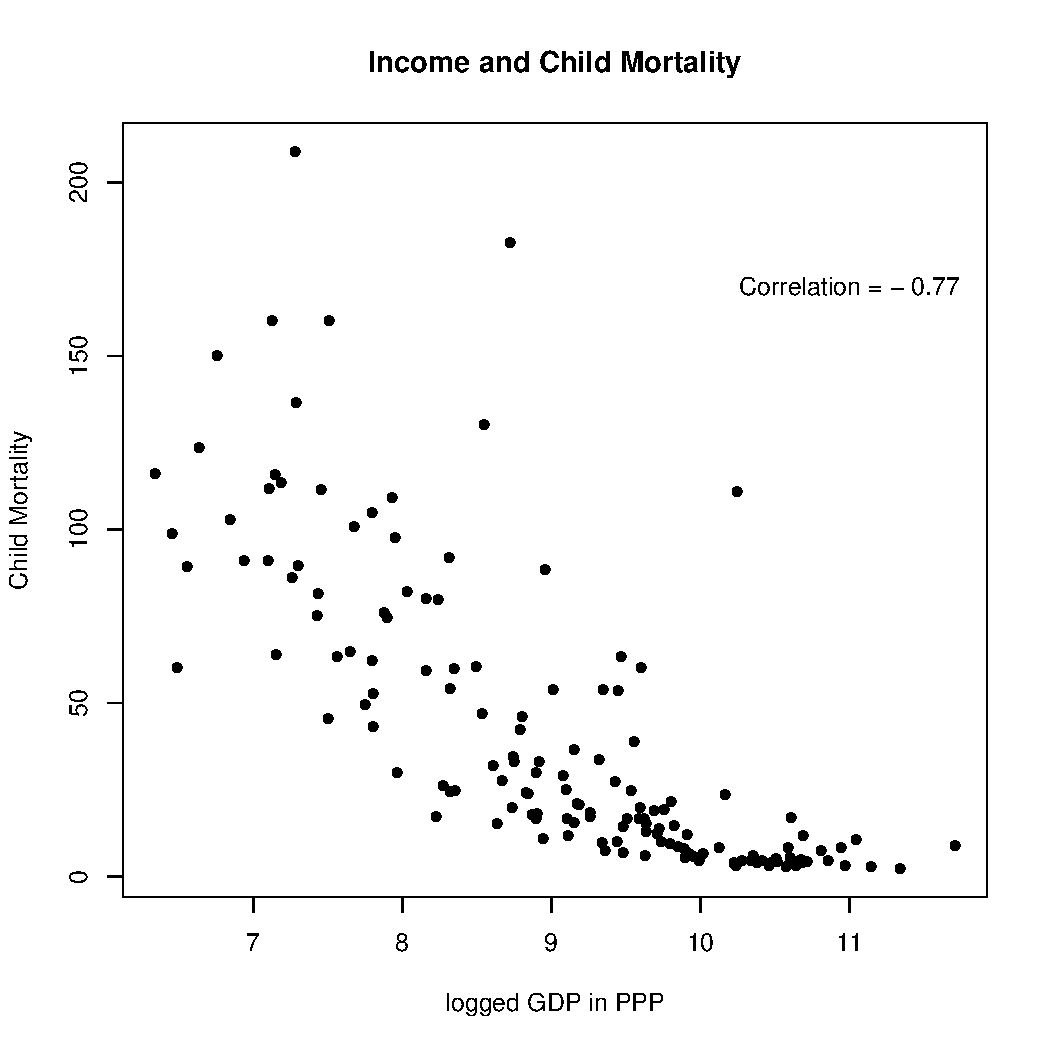
\includegraphics[width=6cm]{/Users/florianhollenbach/Documents/GitHub/Polisci209_2018/slides/week7/scatter_cor.pdf}
\end{center}

\alert{What is the correlation?}
\end{frame}

\begin{frame}[label={sec:org4e7baf3}]{Recall the definition of correlation}
Correlation (x,y) \(= \frac{1}{N} \sum^{N}_{i=1}\) z-score of \(x_i \times\) z-score of \(y_{i}\)

Correlation (x,y) \(= \frac{1}{N} \sum^{N}_{i=1} \frac{x_{i} - \bar{x}}{sd_{x}} \times   \frac{y_{i} - \bar{y}}{sd_{y}}\)
\end{frame}


\begin{frame}[label={sec:org52087f5}]{Correlations \& Scatterplots/Data points}
\begin{enumerate}
\item positive correlation \(\rightsquigarrow\) upward slope
\item negative correlation \(\rightsquigarrow\) downward slope
\item high correlation \(\rightsquigarrow\) tighter, close to a line
\item correlation \alert{cannot} capture nonlinear relationship
\end{enumerate}
\end{frame}

\begin{frame}[label={sec:org4a9ee8b}]{Correlations \& Scatterplots/Data points}
\begin{center}
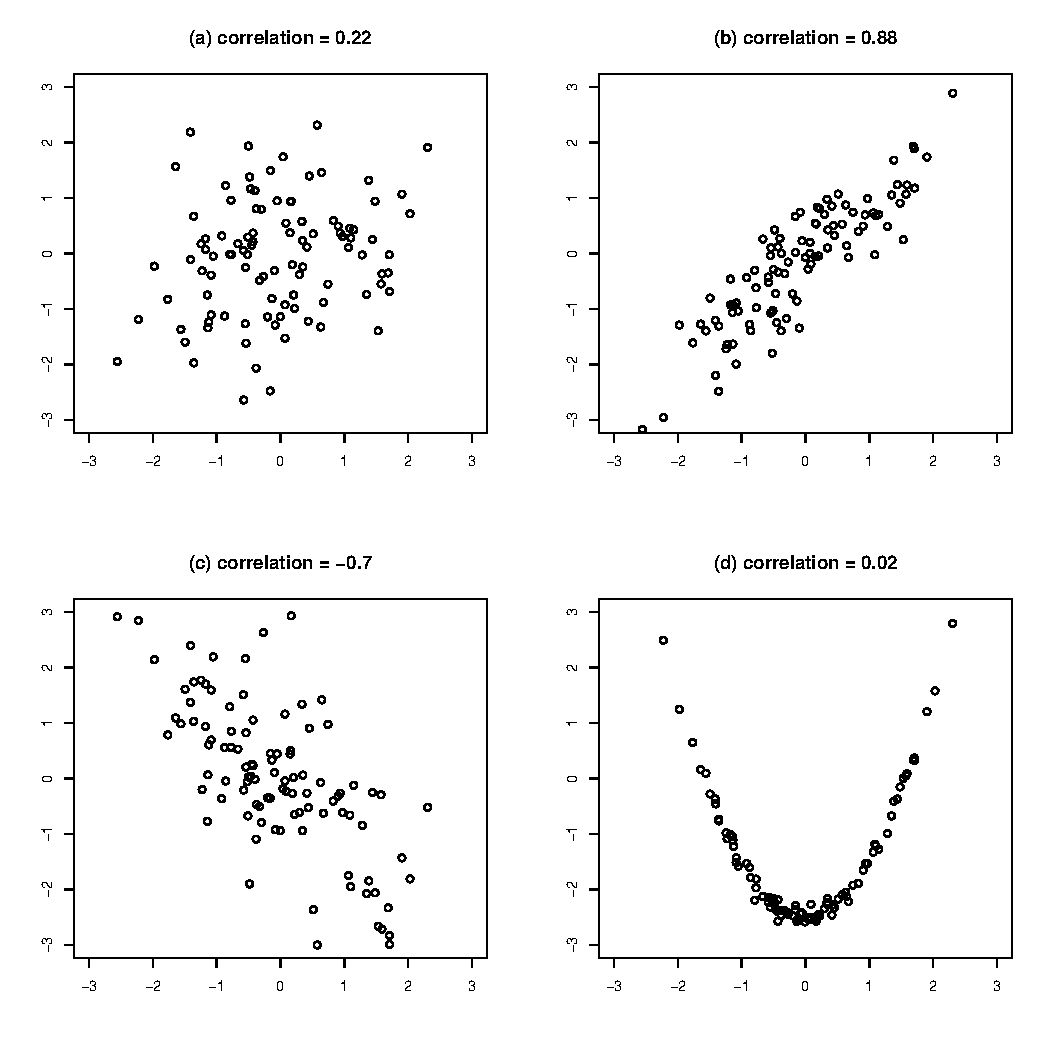
\includegraphics[width=8cm]{/Users/florianhollenbach/Documents/GitHub/Polisci209_2018/slides/week7/correlations.pdf}
\end{center}
\end{frame}


\begin{frame}[label={sec:org35165c8}]{Moving from Correlation to Linear Regression}
Preview:
\begin{itemize}
\item linear regression allows us to create predictions
\item linear regression specifies direction of relationship
\item linear regression allows us to examine more than two variables at the same time (\emph{statistical control})
\end{itemize}
\end{frame}

\begin{frame}[label={sec:orgfc27ab3}]{Linear Regression}
\begin{itemize}
\item regression has one \alert{dependent (y)} and \emph{for now} one \alert{independent (x)} variable
\item regression is a statistical method to estimate the linear relationship between variables
\end{itemize}
\end{frame}

\begin{frame}[label={sec:org09cdda7}]{Linear Regression}
\begin{itemize}
\item goal of regression is to approximate the (linear) relationship between X and Y as best as possible
\end{itemize}
\pause
\begin{itemize}
\item regression is the mathematical model to draw best fitting line through cloud of points
\end{itemize}
\end{frame}


\begin{frame}[label={sec:org4b86b6d}]{Linear Regression}
\begin{center}
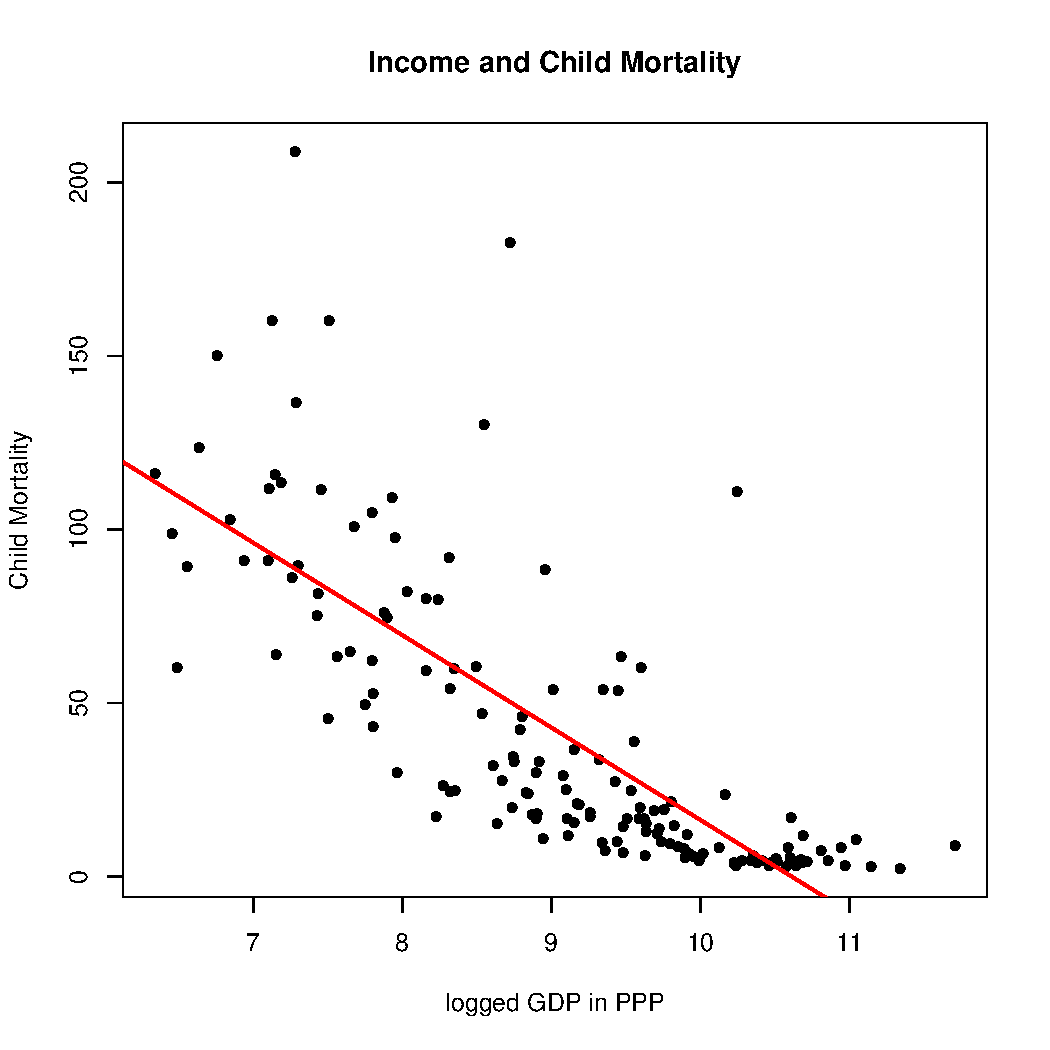
\includegraphics[width=5cm]{/Users/florianhollenbach/Documents/GitHub/Polisci209_2018/slides/week7/scatter_lm.pdf}
\end{center}

\alert{Linear regression is the mathematical model to draw best fitting line through cloud of points}
\end{frame}



\begin{frame}[label={sec:org1e2d126}]{Linear Regression}
\begin{center}
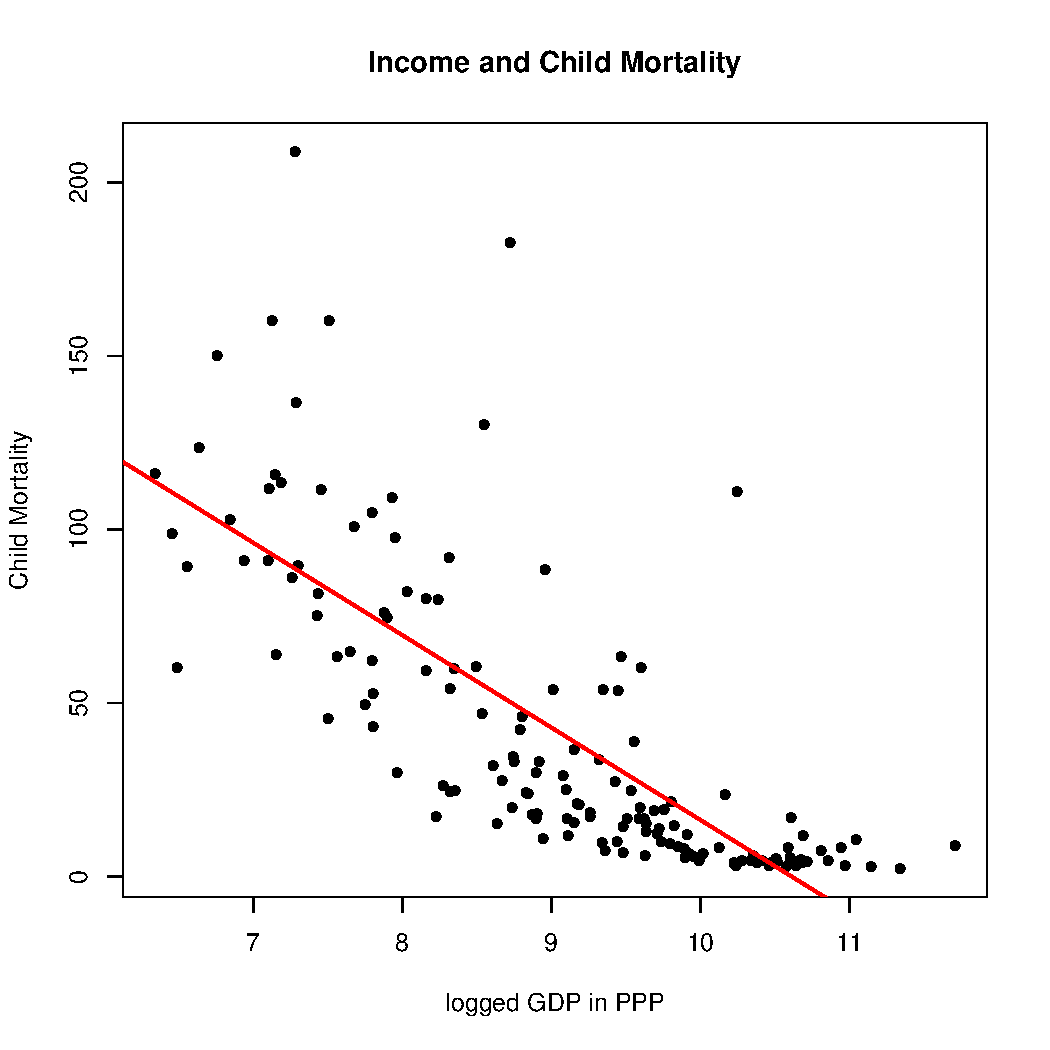
\includegraphics[width=4cm]{/Users/florianhollenbach/Documents/GitHub/Polisci209_2018/slides/week7/scatter_lm.pdf}
\end{center}

\begin{itemize}
\item regression line is an estimate of the (for now bivariate) relationship between x and y
\item for each x we have a prediction of y: \alert{what would we expect y to be given the value of x?}
\end{itemize}
\end{frame}


\begin{frame}[label={sec:orgb9638e4}]{What is the equation of a line?}
\alert{Equation of a line?}
\pause
\(y = m  x + b\)

\(\rightarrow\) b? m?
\end{frame}


\begin{frame}[label={sec:org18ac7d3}]{What is the equation of a line?}
\alert{Equation of a line?}

\(y = m  x + b\)

b \(\rightarrow\) y-intercept

m \(\rightarrow\) slope

\pause

\alert{regression equation:}

\(Y = \alpha + \beta  X + \epsilon\)

\(\rightarrow\) \(\alpha\)? \(\beta\)? \(\epsilon\)?
\end{frame}


\begin{frame}[label={sec:org11dfae2}]{What is the equation of a line?}
\alert{Equation of a line?}

\(y = m  x + b\)

b \(\rightarrow\) y-intercept

m \(\rightarrow\) slope


\alert{regression equation:}

\(Y = alpha + \beta  X + \epsilon\)

\(\alpha\) \(\rightarrow\) y-intercept

\(\beta\) \(\rightarrow\) slope

\(\epsilon\) \(\rightarrow\) error
\end{frame}


\begin{frame}[label={sec:orgfcc614c}]{Regression equation}
\begin{center}
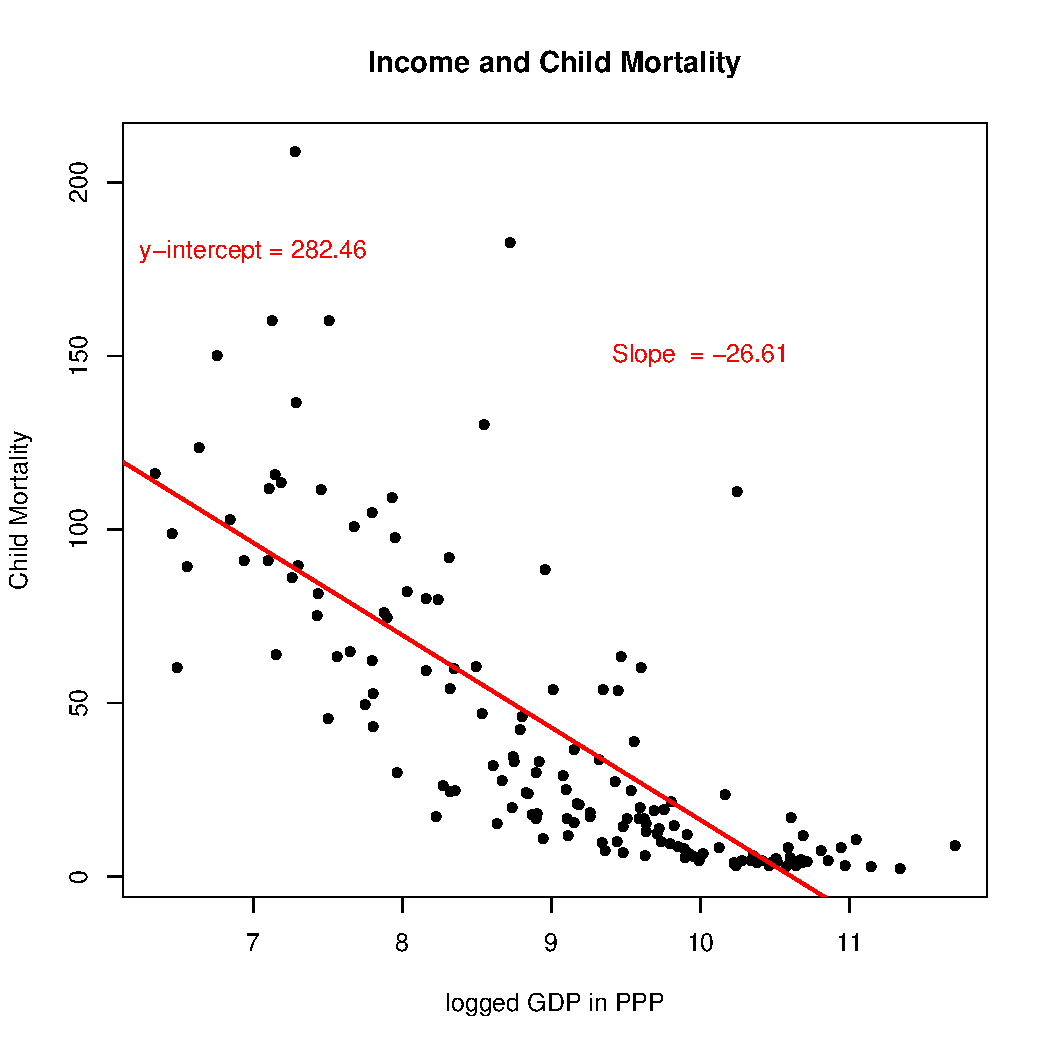
\includegraphics[width=7cm]{/Users/florianhollenbach/Documents/GitHub/Polisci209_2018/slides/week7/scatter_lm_text.pdf}
\end{center}
\end{frame}



\begin{frame}[label={sec:orgaf264c4}]{Regression equation}
\begin{center}
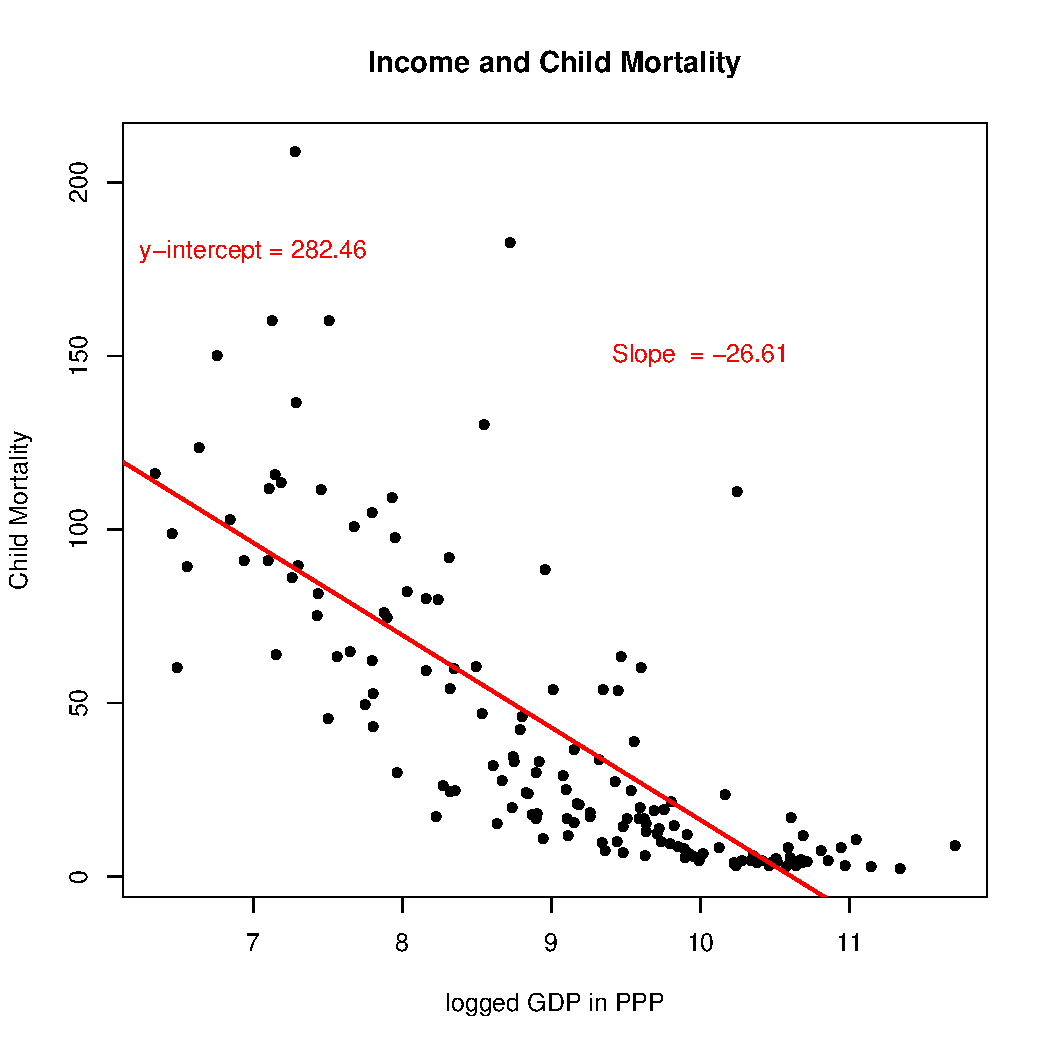
\includegraphics[width=5cm]{/Users/florianhollenbach/Documents/GitHub/Polisci209_2018/slides/week7/scatter_lm_text.pdf}
\end{center}

\(Y = 282.46 + -26.61  X + \epsilon\)
\end{frame}



\begin{frame}[label={sec:org188f648}]{Regression equation}
Model:
\begin{eqnarray*}
    Y & = & \underbrace{\alpha}_{\textsf{intercept}} +
            \underbrace{\beta}_{\textsf{slope}}  X +
            \underbrace{\epsilon}_{\textsf{error term}} \label{eq:linear.model}
  \end{eqnarray*}

\begin{itemize}
\item \(Y\): dependent/outcome/response variable
\item \(X\): independent/explanatory variable, predictor
\item \((\alpha, \beta)\): coefficients (parameters of the model)
\item \(\epsilon\): unobserved error/disturbance term (mean zero)
\end{itemize}
\end{frame}

\begin{frame}[label={sec:org732b66c}]{Regression: Interpretation of the Parameters:}
\begin{eqnarray*}
      Y & = & \underbrace{\alpha}_{\textsf{intercept}} +
              \underbrace{\beta}_{\textsf{slope}}  X +
              \underbrace{\epsilon}_{\textsf{error term}} \label{eq:linear.model}
\end{eqnarray*}

\begin{itemize}
\item \(\alpha + \beta X\): average of \(Y\) at the given the value of \(X\)
\item \(\alpha\): the value of \(Y\) when \(X\) is zero
\item \(\beta\): increase in \(Y\) associated with one unit increase in \(X\)
\end{itemize}
\end{frame}


\begin{frame}[label={sec:org1cbd01e}]{Regression equation}
\begin{itemize}
\item but, we don't know the equation that generates the data
\item our regression line is an estimate, based on the collected data
\end{itemize}

\pause

\begin{itemize}
\item estimates are denoted with little hats: \(\hat{\beta}\), \(\hat{\alpha}\)
\item \((\hat\alpha, \hat\beta)\): estimated coefficients
\end{itemize}

\pause
\begin{itemize}
\item we can use \((\hat\alpha, \hat\beta, X)\) to create \emph{predicted values} of y
\item \(\widehat{Y} = \hat\alpha + \hat\beta x\): predicted/fitted value
\end{itemize}
\end{frame}


\begin{frame}[label={sec:orga31a047}]{Regression equation}
\Large{How far off is our line? How do we know?}
\end{frame}


\begin{frame}[label={sec:org0790a2d}]{Regression equation}
How far off is our line? How do we know?

\pause
\(\hat\epsilon = \text{ true } Y - \widehat{Y}\): residuals/error

\(\hat\epsilon\)'s are an estimate of how good/bad our line approximates the relationship
\end{frame}

\begin{frame}[label={sec:org30e7111}]{Regression}
\begin{center}
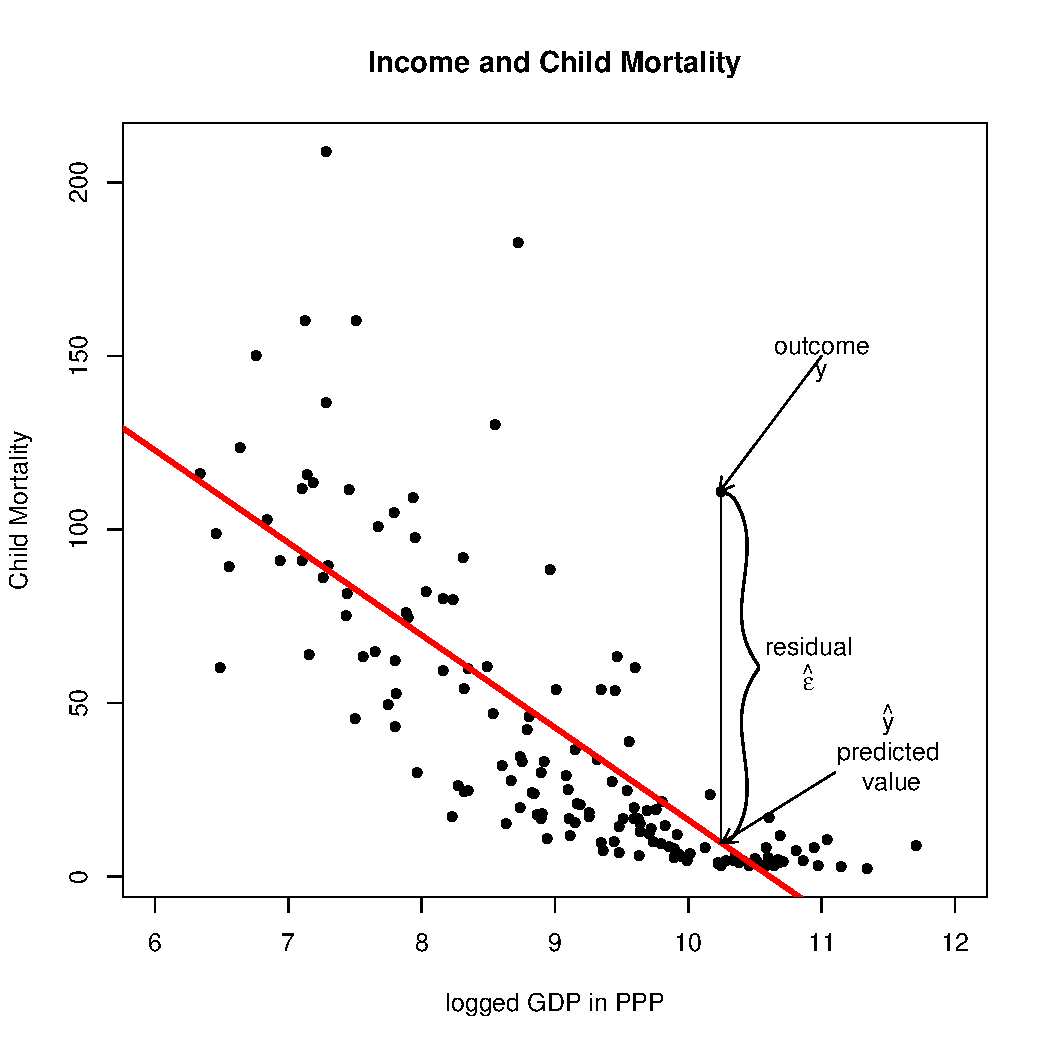
\includegraphics[width=7cm]{/Users/florianhollenbach/Documents/GitHub/Polisci209_2018/slides/week7/scatter_lm_resid.pdf}
\end{center}
\end{frame}



\begin{frame}[label={sec:orgc413d4e}]{Regression}
\begin{itemize}
\item \((\alpha, \beta)\) are estimated from the data
\item How do we find \(\alpha, \beta\)?
\end{itemize}
\end{frame}

\begin{frame}[label={sec:org961fed5}]{Regression: How do we find \(\alpha, \beta\)?}
\alert{We minimize the sum of the squared residuals}

\begin{center}

\includegraphics[width=5cm]{/Users/florianhollenbach/Documents/GitHub/Polisci209_2018/slides/week7/wat.png}
\end{center}
\end{frame}



\begin{frame}[label={sec:orgc16bb9f}]{Regression: How do we find \(\alpha, \beta\)?}
\alert{We minimize the \emph{sum of the squared residuals (SSR)}}

\begin{eqnarray*}
\textsf{SSR} & = & \sum_{i=1}^n \hat\epsilon_i^2
\end{eqnarray*}
\end{frame}

\begin{frame}[label={sec:orgf721f77}]{Regression: How do we find \(\alpha, \beta\)?}
\alert{We minimize the \emph{sum of the squared residuals (SSR)}}

\begin{eqnarray*}
\textsf{SSR} & = & \sum_{i=1}^n \hat\epsilon_i^2
              \ = \ \sum_{i=1}^n (Y_i - \widehat{Y_{i}})^2
\end{eqnarray*}
\end{frame}

\begin{frame}[label={sec:org0750668}]{Regression: How do we find \(\alpha, \beta\)?}
\alert{We minimize the \emph{sum of the squared residuals (SSR)}}

\begin{eqnarray*}
\textsf{SSR} & = & \sum_{i=1}^n \hat\epsilon_i^2
              \ = \ \sum_{i=1}^n (Y_i - \widehat{Y_{i}})^2
              \ = \  \sum_{i=1}^n (Y_i - \hat\alpha - \hat\beta X_i)^2
\end{eqnarray*}

\pause

This also minimizes the root mean squared error: RMSE \(= \sqrt{\frac{1}{n}\textsf{SSR}}\)
\end{frame}

\begin{frame}[label={sec:orgbda93af}]{Regression by Hand}
\begin{eqnarray*}
  \hat\alpha & = & \bar{Y} - \hat\beta \bar{X} \\
  \hat\beta & = & \frac{\sum_{i=1}^n (Y_i - \overline{Y})(X_i - \overline{X})}{\sum_{i=1}^n (X_i - \overline{X})^2}
    \end{eqnarray*}

OR:
\pause
\begin{eqnarray*}
      \hat\beta & = & \textsf{correlation of $X$ and $Y$} \times
                      \frac{\textsf{standard deviation of $Y$}}{\textsf{standard
                      deviation of $X$}}
    \end{eqnarray*}
\end{frame}


\begin{frame}[label={sec:org4f2aad5}]{Regression by Hand}
Regression line always goes through the point of averages (\(\hat{X},\hat{Y}\))

\begin{eqnarray*}
   \widehat{Y}  & = & (\overline{Y} - \hat\beta \overline{X}) + \hat\beta \overline{X} \ =
                    \ \overline{Y}
\end{eqnarray*}
\end{frame}


\begin{frame}[label={sec:orgdab9fa3}]{Regression always goes through point of averages}
\begin{center}
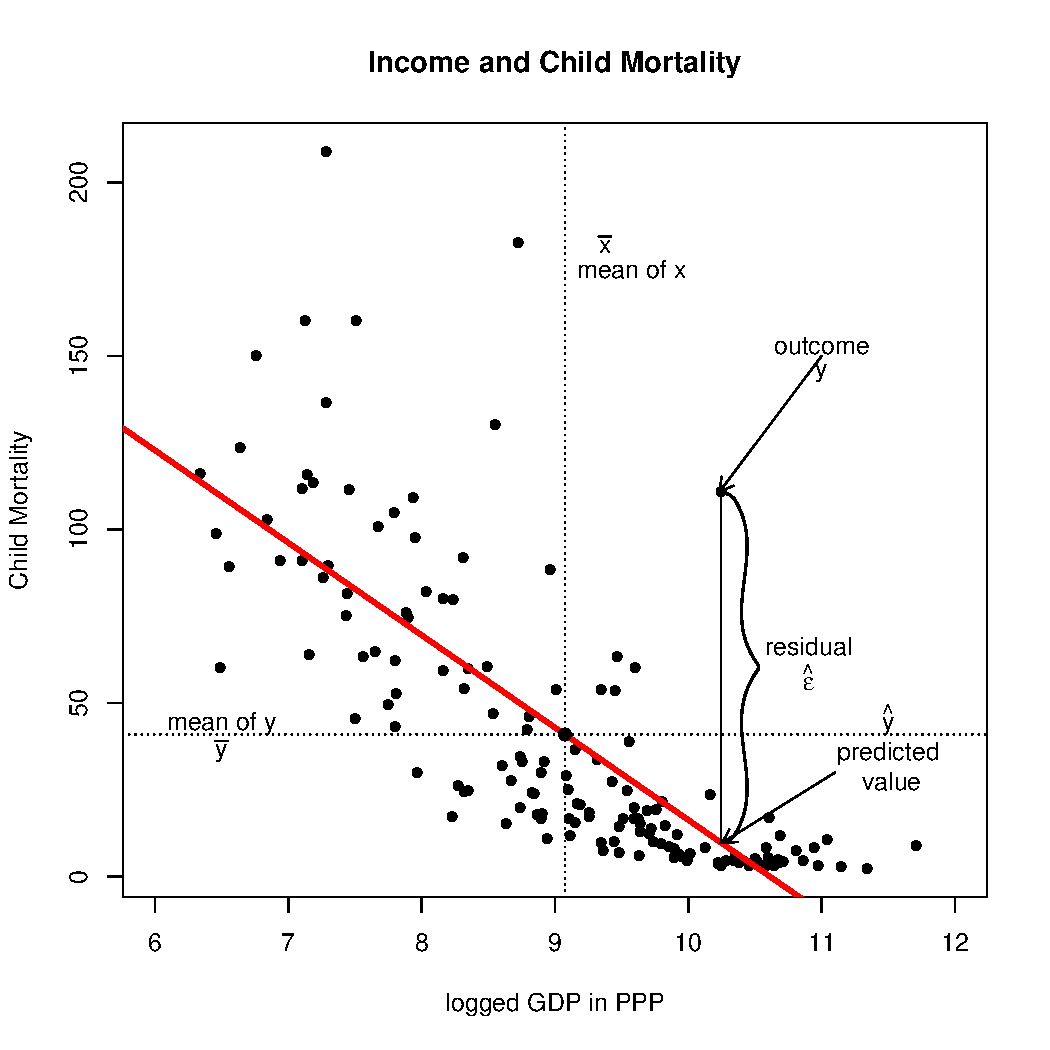
\includegraphics[width=7cm]{/Users/florianhollenbach/Documents/GitHub/Polisci209_2018/slides/week7/scatter_lm_mean.pdf}
\end{center}
\end{frame}


\begin{frame}[fragile,label={sec:org4e9f428}]{Regression NOT by Hand}
 \alert{Enough math!}

Fitting/estimating a regression in \emph{R}:

\begin{verbatim}
lm(dependent ~ independent, data = data_object)
\end{verbatim}
\end{frame}


\begin{frame}[fragile,label={sec:org700a1ad}]{Regression NOT by Hand}
 \alert{Fitting/estimating a regression in \emph{R}:}

\begin{verbatim}
data <- read.csv("bivariate_data.csv")
data <- subset(data, Year ==2010)
result <- lm(Child.Mortality ~ log(GDP) , data = data)
summary(result)
\end{verbatim}
\end{frame}


\begin{frame}[fragile,label={sec:org93b4a79}]{Regression NOT by Hand}
 \begin{verbatim}
result <- lm(Child.Mortality ~ log(GDP) , data = data)
coef(result) ### coefficients
\end{verbatim}

\begin{verbatim}

(Intercept)    log(GDP) 
  282.45870   -26.61347
\end{verbatim}

\emph{R}-output:

(Intercept): \(\alpha\)

\emph{log(GDP)}: \(\beta\)
\end{frame}

\begin{frame}[label={sec:org8d84d55}]{Model Fit}
How well does our regression line fit the data?

How well does the model predict the outcome?

\pause

\(R^{2}\) or \emph{coefficient of determination}:

\begin{eqnarray*}
      R^2 & = & 1 - \frac{\textsf{SSR}}{\textsf{Total sum of squares (TSS)}}  \ = \ 1 - \frac{\sum_{i=1}^n \hat\epsilon_i^2}{\sum_{i=1}^n (Y_i - \overline{Y})^2}
    \end{eqnarray*}
\end{frame}

\begin{frame}[label={sec:org882112c}]{Model Fit}
\begin{eqnarray*}
      R^2 & = & 1 - \frac{\textsf{SSR}}{\textsf{Total sum of squares (TSS)}}  \ = \ 1 - \frac{\sum_{i=1}^n \hat\epsilon_i^2}{\sum_{i=1}^n (Y_i - \overline{Y})^2}
    \end{eqnarray*}

\(R^{2}\) is also defined as the \emph{explained variance} in Y

How much of the deviation of Y from the average is explained by X?
\end{frame}



\begin{frame}[fragile,shrink=15,label={sec:orgf8d2db1}]{Model Fit}
 \begin{verbatim}
result <- lm(Child.Mortality ~ log(GDP) , data = data)
summary(result)
\end{verbatim}

\begin{verbatim}

Call:
lm(formula = Child.Mortality ~ log(GDP), data = data)

Residuals:
    Min      1Q  Median      3Q     Max 
-49.455 -15.418  -4.161  10.847 132.136 

Coefficients:
            Estimate Std. Error t value Pr(>|t|)    
(Intercept)  282.459     16.569   17.05   <2e-16 ***
log(GDP)     -26.613      1.809  -14.71   <2e-16 ***
---
codes:  0 ‘***’ 0.001 ‘**’ 0.01 ‘*’ 0.05 ‘.’ 0.1 ‘ ’ 1

Residual standard error: 27.57 on 150 degrees of freedom
Multiple R-squared:  0.5906,	Adjusted R-squared:  0.5878 
F-statistic: 216.4 on 1 and 150 DF,  p-value: < 2.2e-16
\end{verbatim}
\end{frame}
\end{document}